\documentclass[tikz]{standalone}
\usetikzlibrary{positioning}
\usepackage{makecell}

\begin{document}

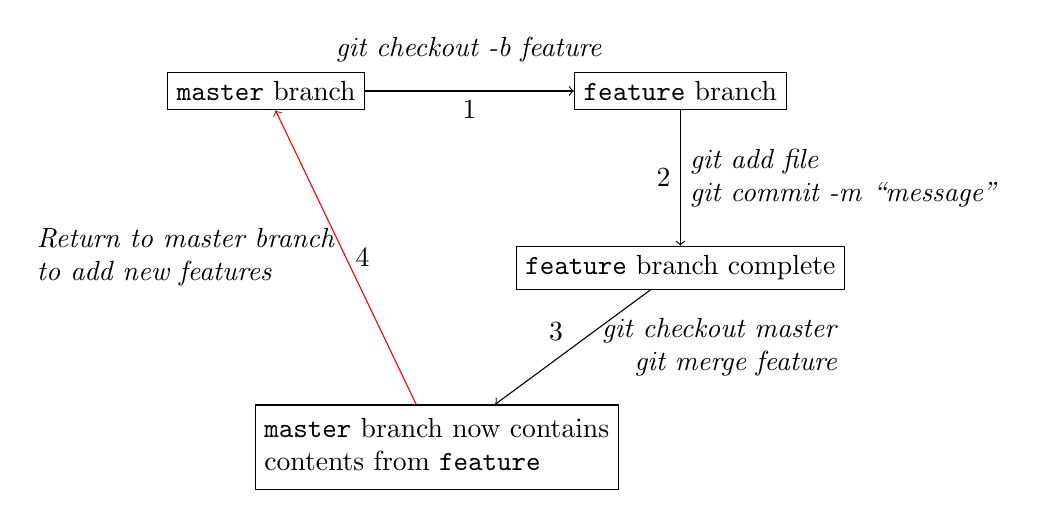
\begin{tikzpicture}
	\node[] at (0, 0) [rectangle,draw] (master) {\texttt{master} branch};
	\node[] at ([xshift=4cm]master.east) [rectangle,draw] (feature) {\texttt{feature} branch};
	\draw[->] (master)  -- node[below]{1} node[yshift=0.25cm,above] {\emph{git checkout -b feature}} (feature);
	\node[] at ([yshift=-2cm]feature.south) [rectangle,draw] (featuredone) {\texttt{feature} branch complete};
	\draw[->] (feature)  -- node[left]{2} node[right] {\makecell[l]{\emph{git add file}\\\emph{git commit -m ``message"}}} (featuredone);
	\node[] at ([xshift=-1cm,yshift=-2cm]featuredone.south west) [rectangle,draw] (merged) {\makecell[l]{\texttt{master} branch now contains\\contents from \texttt{feature}}};
	\draw[->] (featuredone) -- node[yshift=2mm,left]{3} node[xshift=0.25cm,right] {\makecell[r]{\emph{git checkout master}\\\emph{git merge feature}}} (merged);
\draw[->,draw=red] (merged) -- node[right]{4} node[left]{\makecell[l]{\emph{Return to master branch}\\\emph{to add new features}}} (master);
\end{tikzpicture}

\end{document}
